\documentclass[a4paper,11pt]{article}

\usepackage{style}

\begin{document}
\newtitle{Extracting cognitive brain networks using machine-learning and information theoretical approaches}{Research report}


% ______________________________ INTRODUCTION ______________________________

\section*{Abbreviations}
\begin{flushleft}
    % \begin{footnotesize}
        \begin{multicols}{2}
            \begin{singlespace}
                \printacronyms[heading=none]
            \end{singlespace}
        \end{multicols}
    % \end{footnotesize}
\end{flushleft}
    

\section{Introduction}

\begin{multicols}{2}

% Keywork to include in the intro :
% \begin{enumerate}
%     \item Humans and \ac{ieeg}
%     \item Local, network, cognition
%     \item Machine-learning, Information-theory, Statistics
% \end{enumerate}






What is the functional unit of the brain?

Global introduction on my view of the brain... The brain from the inside out?

My present research focus on the \textbf{discovery of cognitive brain networks}, especially during learning, using human \ac{ieeg}. This involves working at two different spatial scales : a \textbf{local scale} where I try to identify computations performed in brain regions that are driven by the behaviour of the subject or by external stimulations. The second scale consists in understanding the role of \textbf{network} modulations i.e. 

My work is located at the border 



WHY DID I SWITCH TO IT????
- Support heterogene data (continuous / discrete)
- Framework (Ince)
- Model-free
- Show the strong link with hospitals for recordings iEEG???

====================== SHOW EXPLAIN NOVELTY =================



\paragraph{Background :}

\paragraph{Thesis :} I did my PhD thesis under the co-supervision of Prof. Aymeric Guillot at the \textit{Laboratoire Interuniversitaire de Biologie de la Motricité} in Lyon and Prof. Karim Jerbi at the \textit{Computational and Cognitive Neuroscience Lab} in the University of Montreal.

\paragraph{Postdocs :} I did two postdocs...

\paragraph{Present :} My present research focus on...

\paragraph{Scientific contributions :}

This is me.

\end{multicols}



% _____________________________ LOCAL ENCODING _____________________________


\section{Decoding human upper-limp movements}

\begin{highlights}{Highlights}
    WHAT THIS SECTION BRING AS NOVELTY ----------------------- >
    \begin{description}
        \item[2017 :] We used \ac{ml} approaches to decode whether human subjects were \textbf{planning or executing upper-limb movements} using \ac{ieeg}. We compared the decoding performance of local spectral markers.
        \item[Preliminary :] We showed that we can infer \textbf{upper-limb movement directions while planning and executing} and both motor states shared similar representations
        \item[2020 :] We proposed a method for measuring \ac{cfc} using metrics from the \ac{it}
    \end{description}
\tcblower
\cite{combrisson2017intentions,combrisson2020tensorpac}, Combrisson et al., \textit{in prep}
\end{highlights}

\begin{multicols}{2}

Executing simple movement is associated to complex but reproducible neural patterns in the oscillatory activity of the brain. As an example, both invasive and non-invasive brain recordings reported in the motor cortex a relative increase and decrease in the high-frequency and beta band power respectively while executing hand movements. \Ac{bci} are devices translating those neural patterns into commands used to restore the communication or a partial mobility to, for example, patients with locked-in syndrome. Hence, characterizing those patterns contribute both to the fundamental understanding of the brain and also has a direct clinical application. However, our understanding of the specific role of neural components such as the amplitude, the phase, or \ac{cfc} mechanisms is still in his infancy.
The goal of my PhD thesis was to address this issue using \ac{ieeg} in epileptic patients performing a center-out motor task. We used \ac{ml} approaches to identify neural markers of \textbf{motor states}, i.e. whether human subjects were either planning or executing hand movements. More ambitiously, we also showed that we could guess with a relatively high accuracy the \textbf{direction of the hand movement} while planning it, i.e. before the actual execution. In addition to the already well-known role of spectral power, this data-driven approach highlighted the important contribution of the low-frequency phase and the \ac{pac}.


% ====================================================================

\subsection{Neural makers of motor states}

\paragraph{\cite{combrisson2017intentions} :} We compared the decoding performance of several neural markers (amplitude, phase and \ac{pac}) to infer the motor state using human \ac{ieeg} recordings \fig{fig_states_decoding}. We retrieved high-decoding performances ($>80\%$) of classical power features in the motor and premotor cortex. However, the best decoding was achieved using the phase in very low frequency band in the premotor cortex ($\sim90\%$). We replicated the existence of an alpha-gamma coupling in the premotor cortex \citep{yanagisawa2012jon} but we showed that it was specific to the planning. Hence, we reported for the first time significant decoding using \ac{cfc} features, suggesting that \ac{bci} devices should explore phase and coupling features.


\end{multicols}

\begin{figure}[H]
\centering
    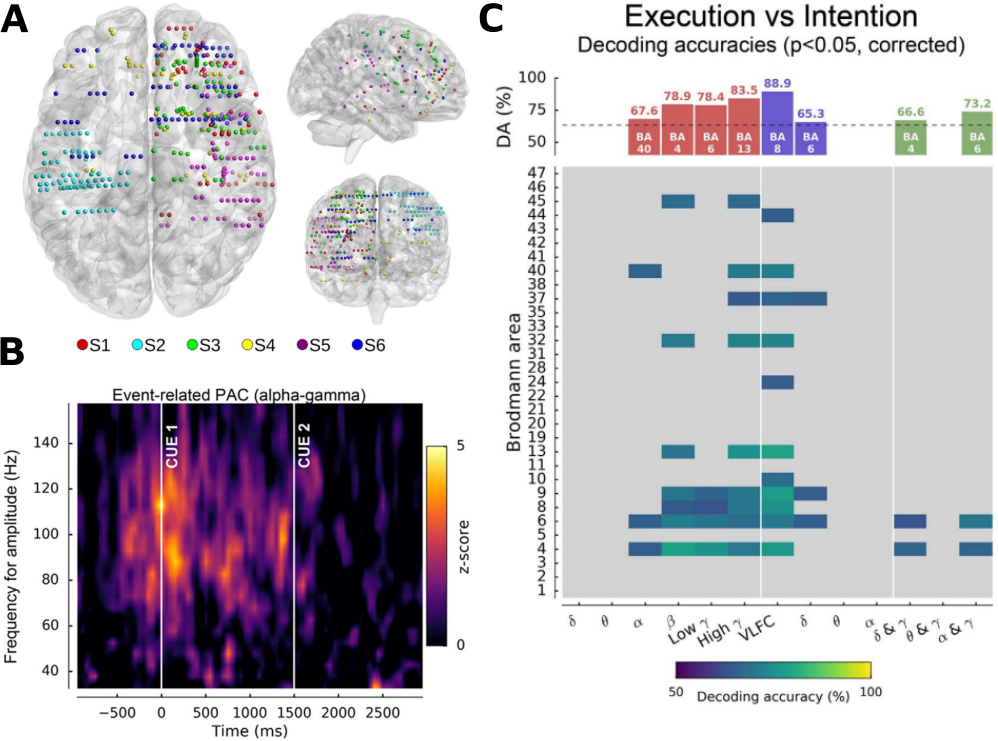
\includegraphics[width=.8\linewidth]{figures/report/combrisson_2017_NI.png}
    \caption{Motor states decoding using amplitude, phase and \ac{pac} neural markers, \textit{(A)} Intracranial implantation of the six subjects \textit{(B)} Event-related alpha-gamma \ac{pac} of a premotor site. The beginning of the planning and execution phases are represented by the two vertical white lines. \textit{(C)} Decoding performances of execution vs. planning. Highest decoding achieved using the \textit{very low frequency phase} ($\sim90\%$)}
    \label{fig_states_decoding}
\end{figure}


% ====================================================================

\begin{multicols}{2}

\subsection{Neural markers of motor direction}

\paragraph{Combrisson et al., \textit{in prep} :} We investigated decoding upper-limb directions (up vs. down vs. right vs. left) using human \ac{ieeg} recordings \fig{fig_dir_decoding}. In comparison to decoding motor states, amplitude features outperformed phase and \ac{pac} markers. In particular, we were able to differentiate the four directions using the alpha power during planning ($\sim44\%$, Fig \ref{fig_dir_decoding}A) and the gamma power during execution ($\sim63\%$, Fig \ref{fig_dir_decoding}B). Using the transfer learning temporal generalization approach \citep{king2014}, we showed that planning and executing a movement shared similar neural representations (Fig \ref{fig_dir_decoding}C). Finally, we used a feature-selection pipeline to combine synergistic features and maximize the decoding performance (Fig \ref{fig_dir_decoding}D). This optimization strategy led to decoding accuracies of the four directions of $\sim75\%$ and $\sim84\%$ respectively during the planning and execution phases. \Ac{pac} markers were equally modulated across-directions, confirming its role in switching in and out of the task.

\end{multicols}

\begin{figure}[H]
\centering
    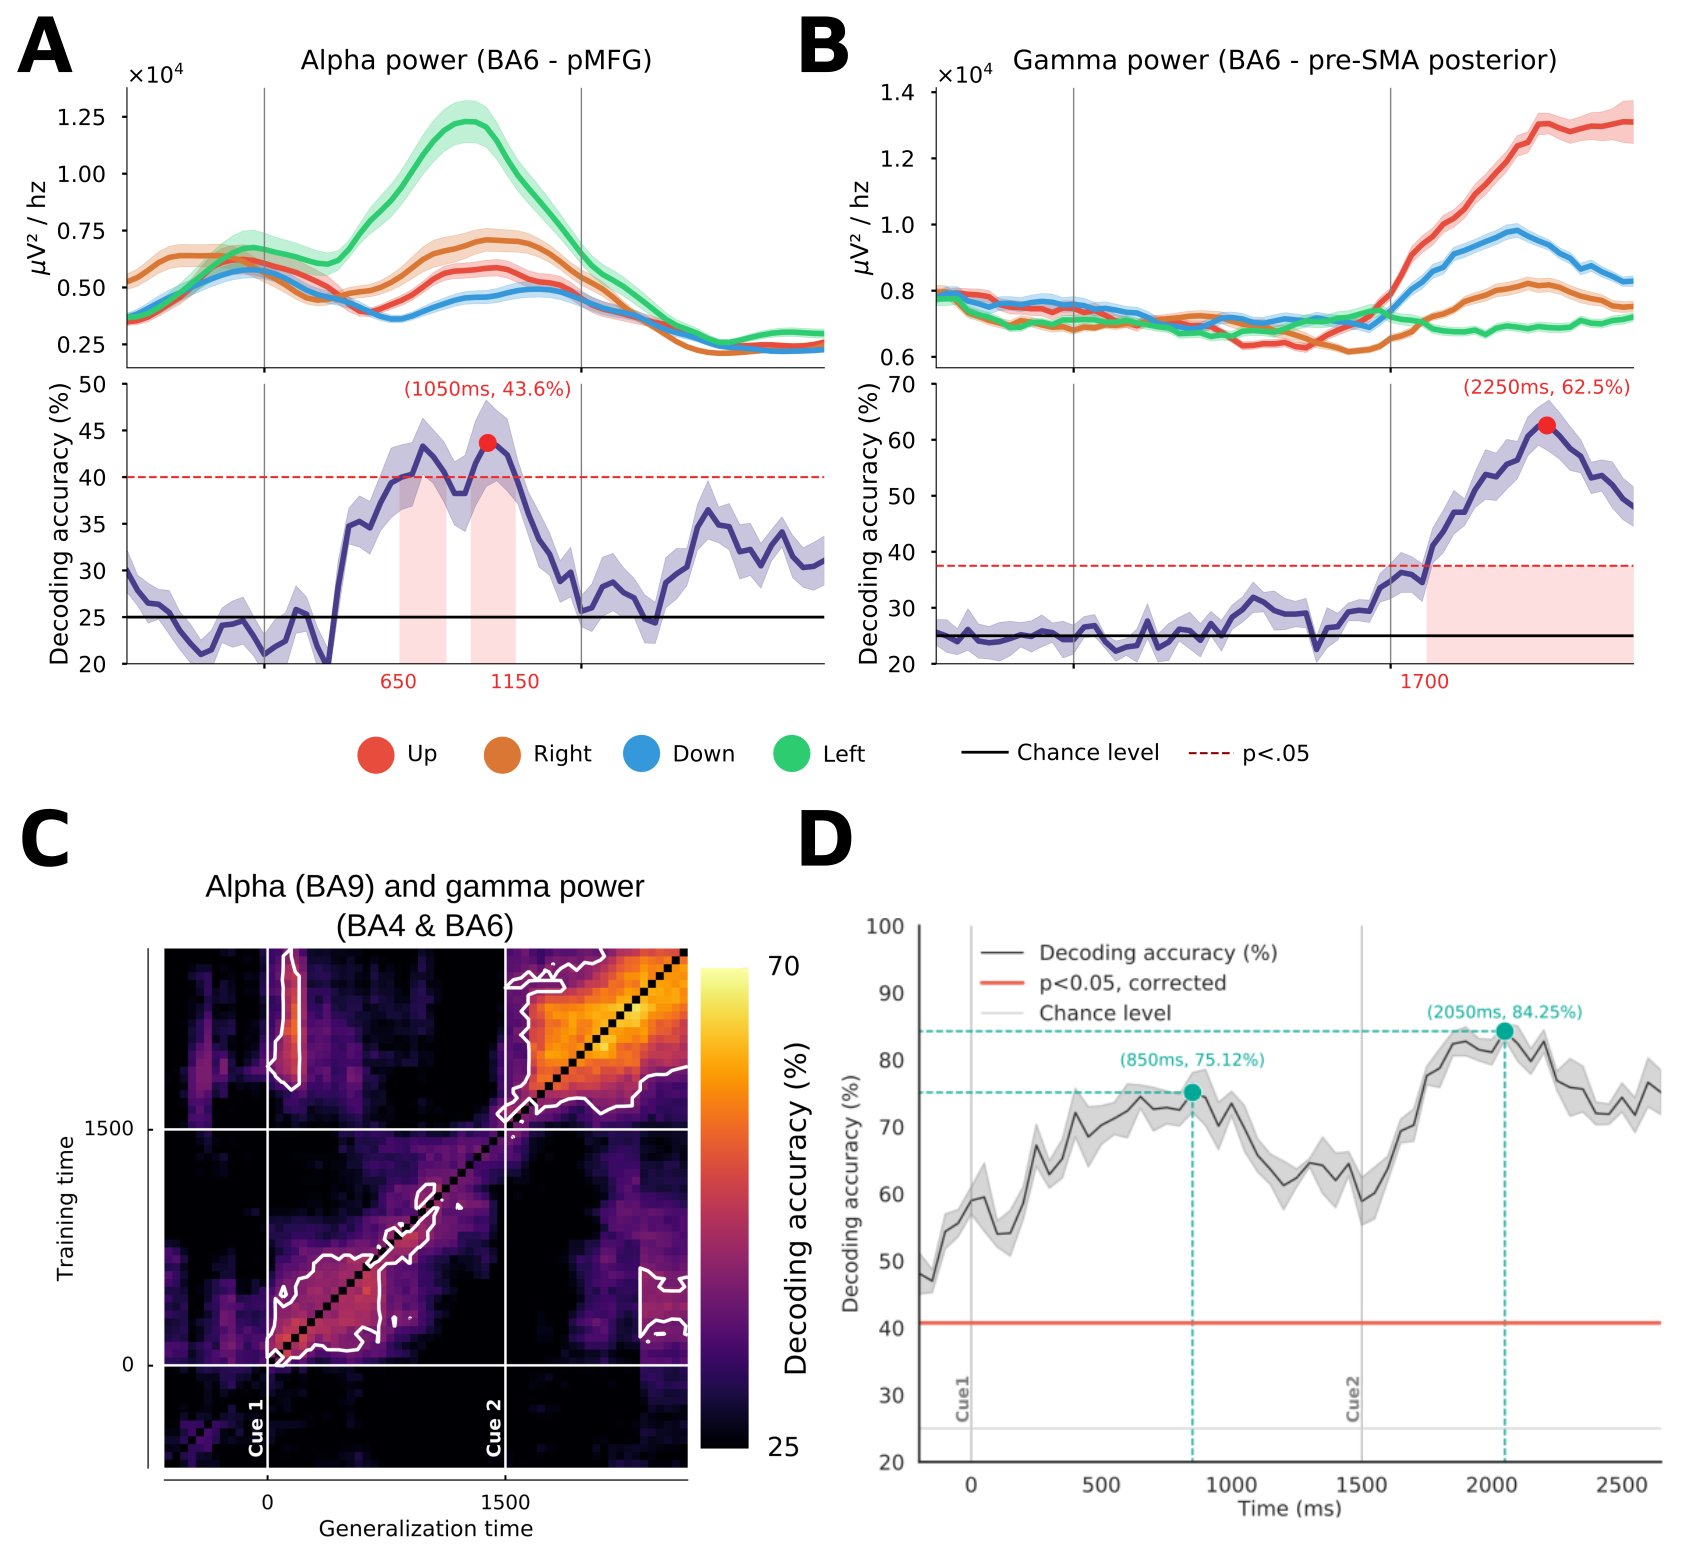
\includegraphics[width=.8\linewidth]{figures/report/combrisson_2030_dir.png}
    \caption{Instantaneous dynamic direction decoding using the \textit{(A)} alpha and \textit{(B)} gamma power of two premotor sites. The top subplot represents the temporal evolution of the power of the four directions (up, right, down and left. The bottom subplot represents the instantaneous decoding of the four directions. \textit{(C)} Temporal generalisation by combining alpha and gamma power features. \textit{(D)} Temporal evolution of the decoding when using a multi-features selection.}
    \label{fig_dir_decoding}
\end{figure}


% ====================================================================

\begin{multicols}{2}

\subsection{Measuring CFC using information-theoretical approaches}

\paragraph{\cite{combrisson2020tensorpac} :} transfer learning temporal generalization

\end{multicols}

% _____________________________ NETWORK ENCODING _____________________________

% \section{Approaching learning as a network emerging property}
\section{Distributed process during learning}




We showed the role of the error monitoring of the insula blablabla \citep{bastin2016direct}. Okokok \citep{gueguen2021anatomical}.

Bastin error monitoring


% _________________________________ STATISTICS _________________________________

% \newpage
\section{Statistical analyses for the discovery of cognitive brain networks}

\begin{highlights}{Highlights}
% \begin{singlespace}
    \begin{description}
        \item[2015 :] We raised a red flag to neuroscientists using \ac{ml} approaches by recalling that the empirical decoding \textbf{chance-level depended on the number of samples}. This paper received great interest and now counts more than 400 citations.
        \item[2022 :] We introduced a statistical framework for performing \textbf{group-level analyses at the local and network levels} using powerful measures of information.
    \end{description}
% \end{singlespace}


\tcblower
\cite{combrisson2015exceeding,combrisson2022grouplevel}

\end{highlights}

WHY PERMUTATIONS ARE IMPORTANT?

% --------------------------------------------------------------------
The discovery of cognitive brain networks relies on 

\subsection{Empirical estimation of the chance level in machine-learning}

For a standard two classes problem, the theoretical chance level i.e. the decoding achievable by chance is 50\%. This theoretical threshold is reachable with an infinite number of samples however, in practice, the decoding chance-level depends on the number of samples and high decoding can be observed with a few samples. 

\begin{wrapfigure}{r}{0.55\textwidth} %this figure will be at the right
    \centering
    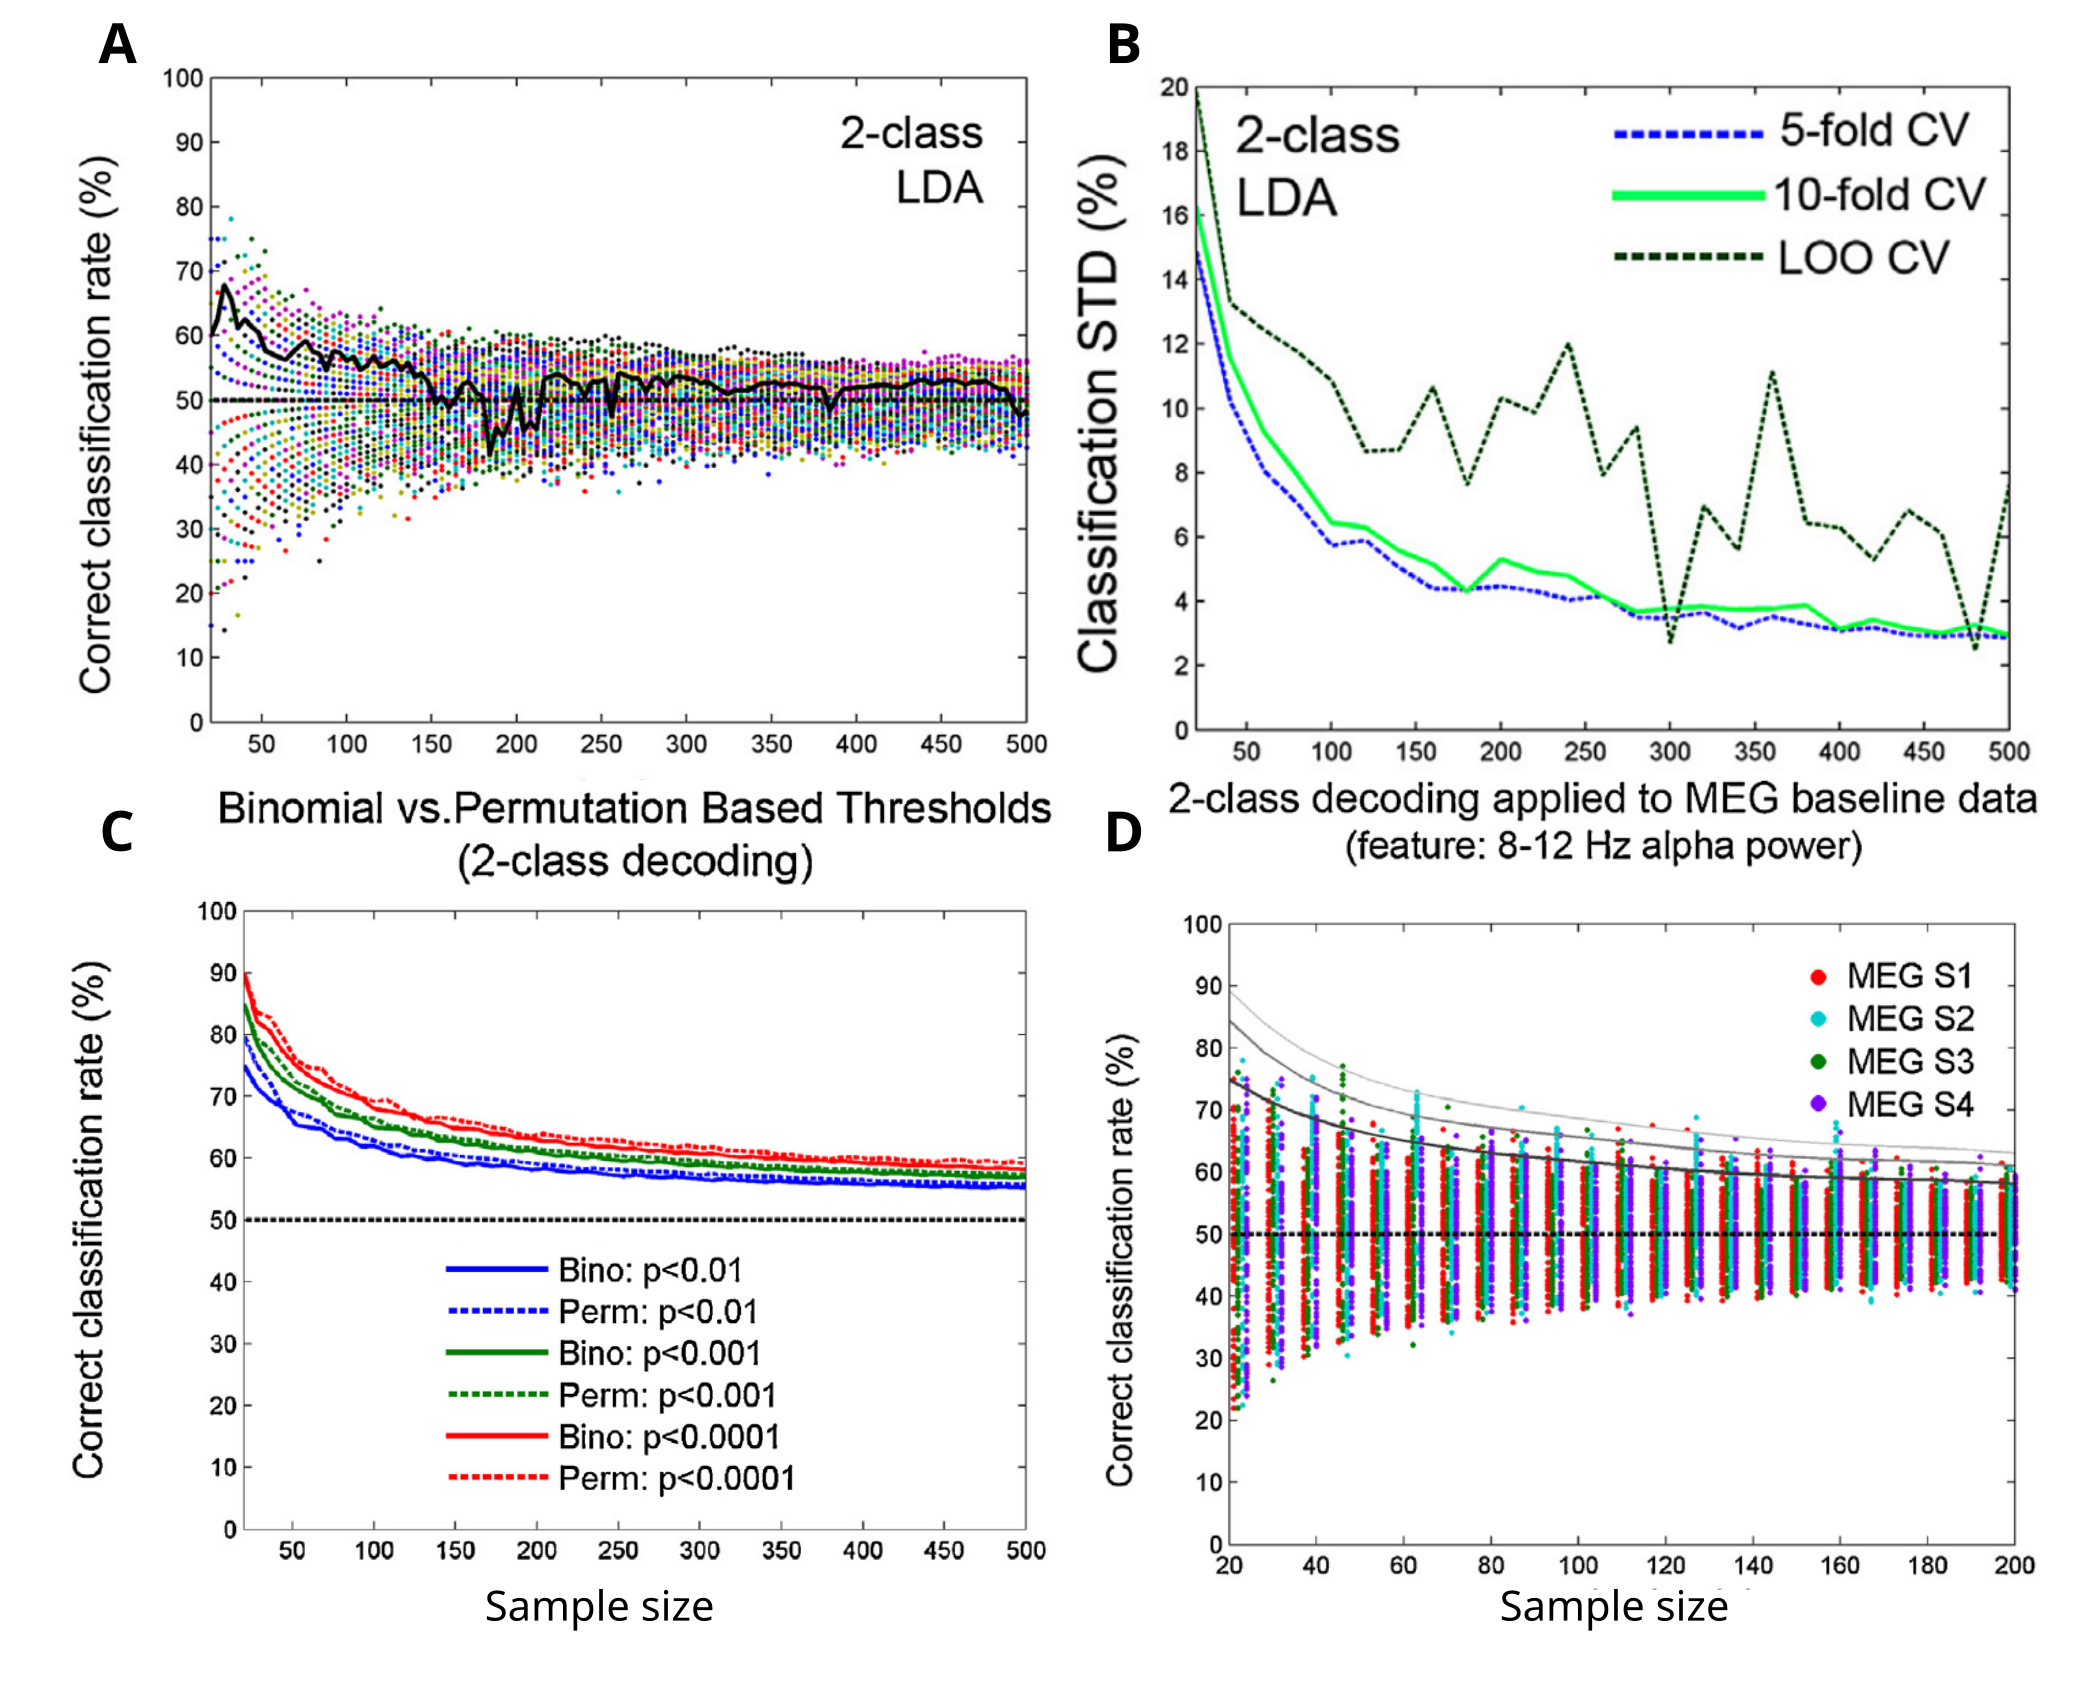
\includegraphics[width=0.55\textwidth]{figures/report/chance_level.png}
    \caption{Dependence of the decoding on the number of samples using \textit{(A)} simulated noise or \textit{(D)} resampled MEG data. This dependence also varies depending on the cross-validation scheme \textit{(B)}. We also compared the statistical threshold obtained using either parametric binomial distributions or a non-parametric permutation-based approach \textit{(C)}.}
    \label{fig_chance_level}
\end{wrapfigure}

The \ac{ml} community was already aware of this dependence on the number of samples, but several neuroscientific studies used this theoretical threshold as a statistical proof of significant decoding. We took this opportunity to raise a red flag by showing this phenomenon \citep{combrisson2015exceeding}. To this end, we classified simulated noise and resampled MEG data with varying number of samples. As expected, we showed that high-decoding could be reached by chance in the presence of a few samples and the more samples there are, the closer the empirical threshold is to the theoretical one \fig{fig_chance_level}. To conclude, we insisted on the use of non-parametric permutations as a data-driven estimation of the chance level.

% \begin{figure}[H]
% \centering
%     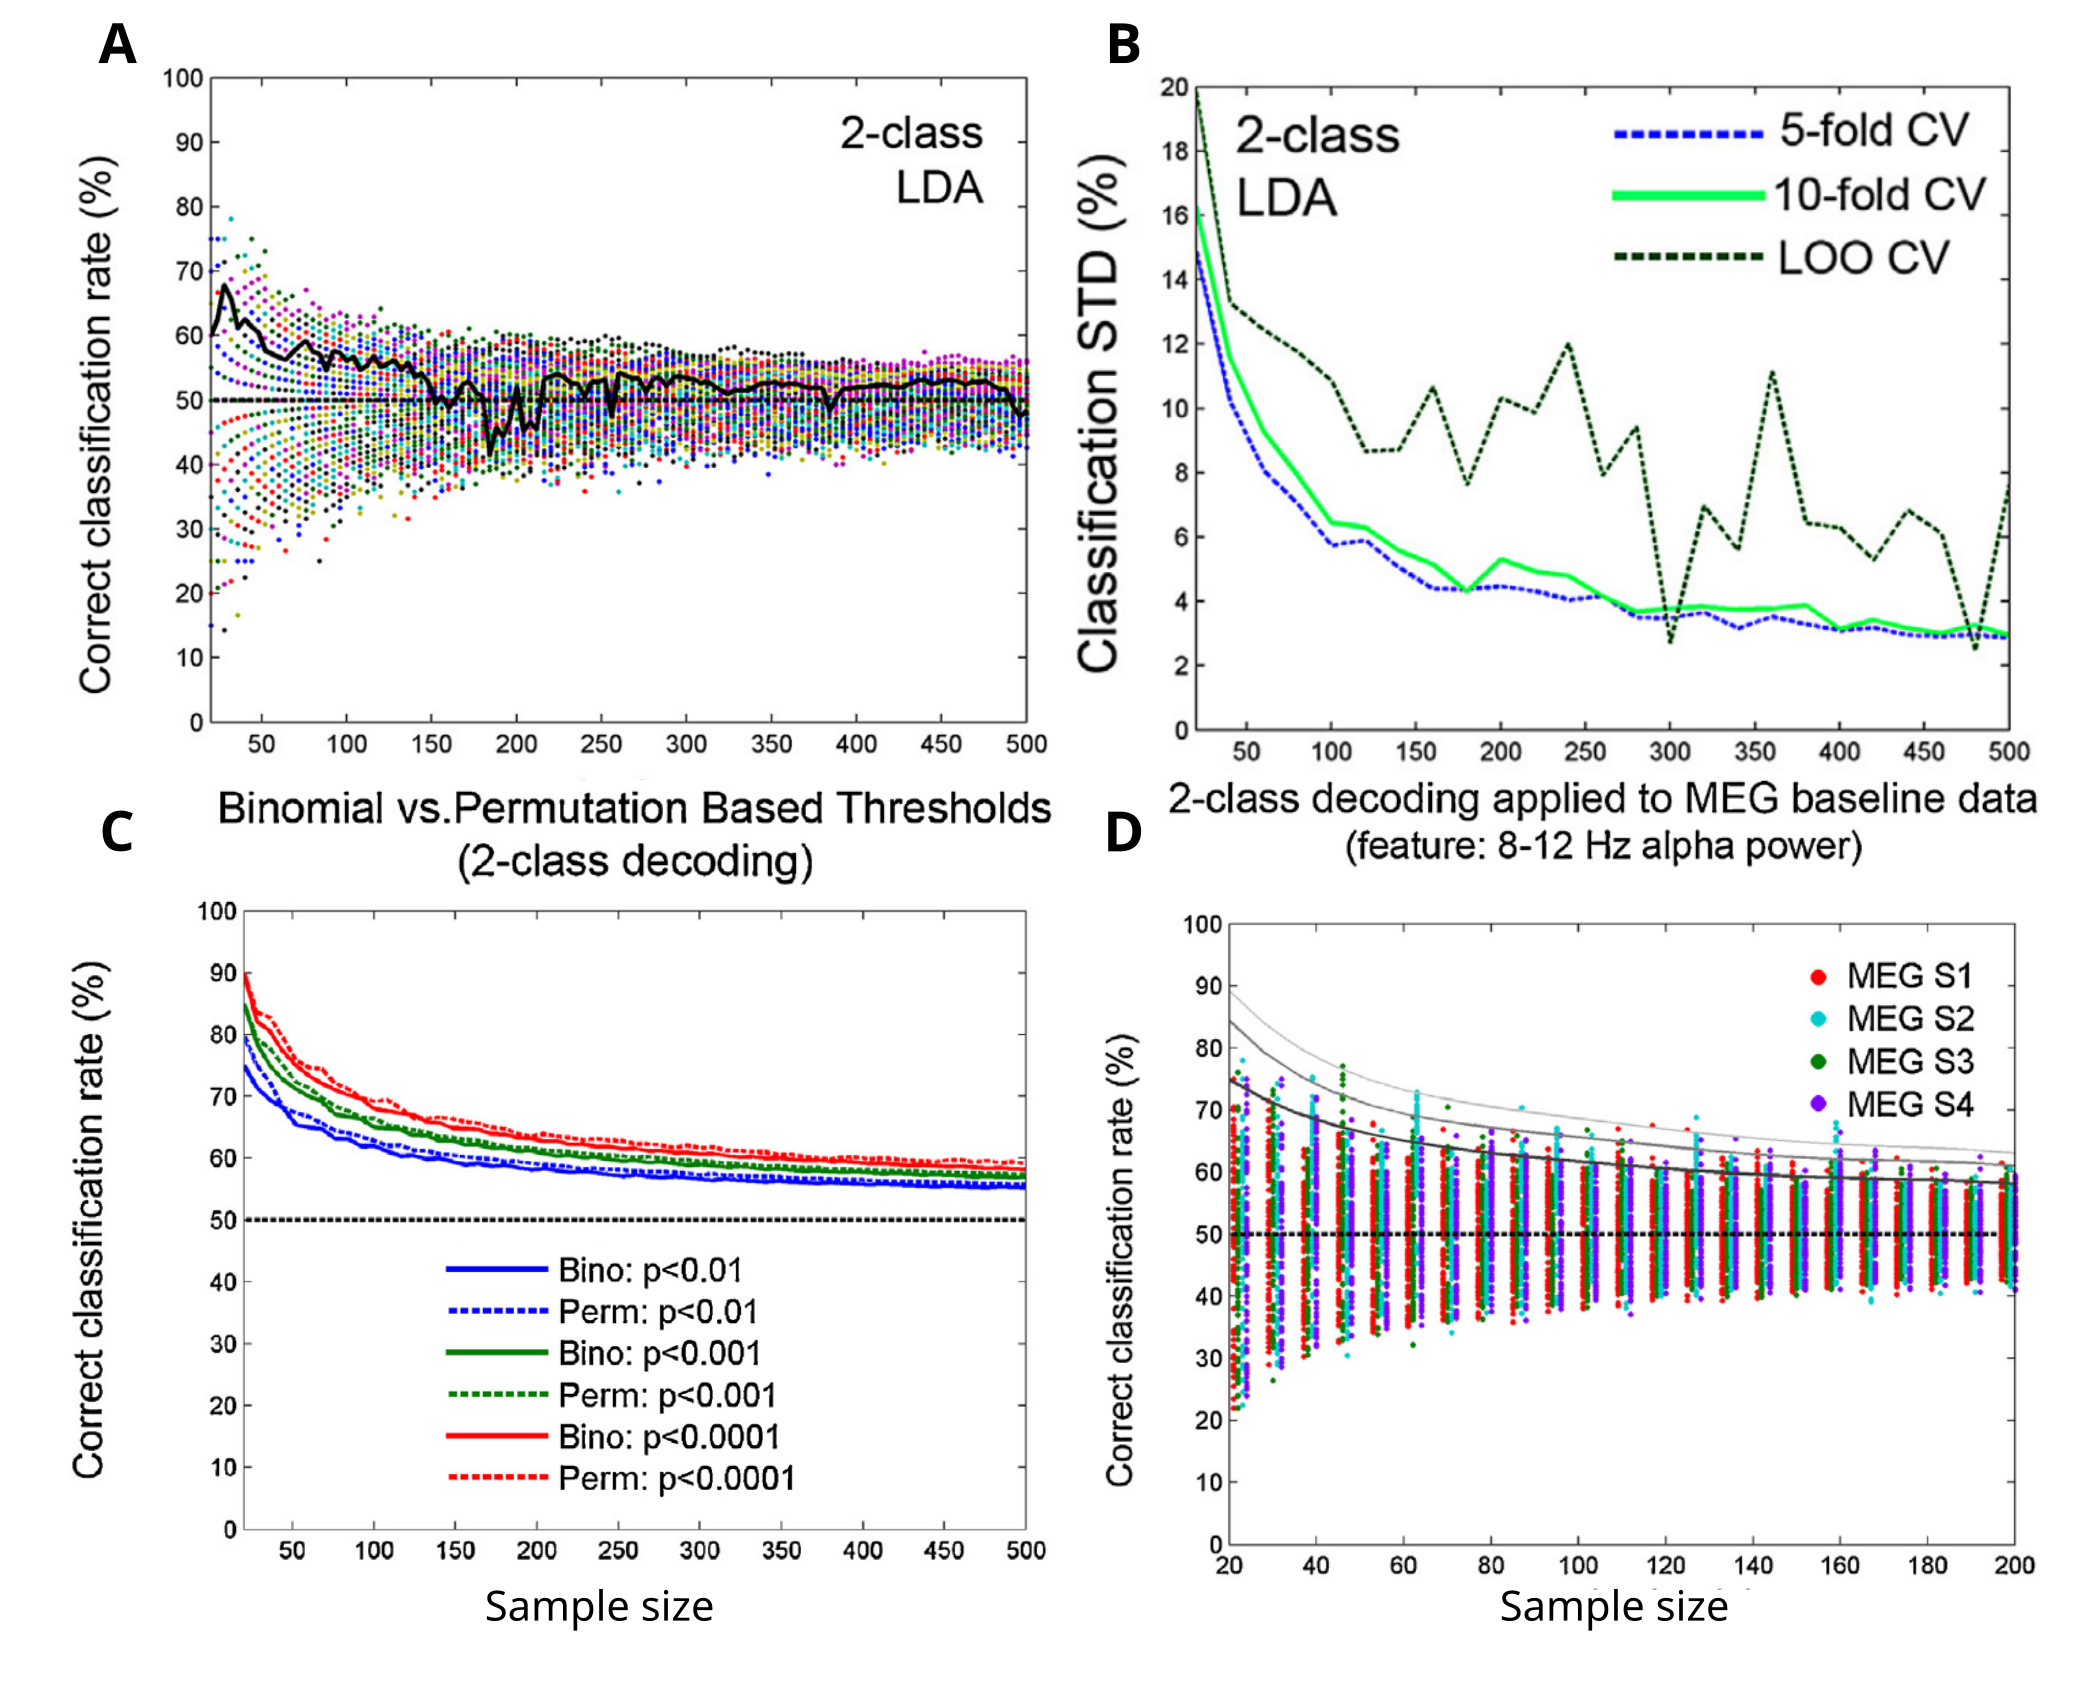
\includegraphics[width=1\linewidth]{figures/report/chance_level.png}
%     \caption{Dependence of the decoding on the number of samples using \textit{(A)} simulated noise or \textit{(D)} resampled MEG data. This dependence also varies depending on the cross-validation scheme \textit{(B)}. We also compared the statistical threshold obtained using either parametric binomial distributions or a non-parametric permutation-based approach \textit{(C)}.}
%     \label{fig_chance_level}
% \end{figure}

% \begin{multicols*}{2}
% [
% \subsection{title}
% ]
% \end{multicols*}

% --------------------------------------------------------------------

\subsection{Group-level inferences at the local and network levels}

\begin{wrapfigure}{r}{0.45\textwidth} %this figure will be at the right
    \centering
    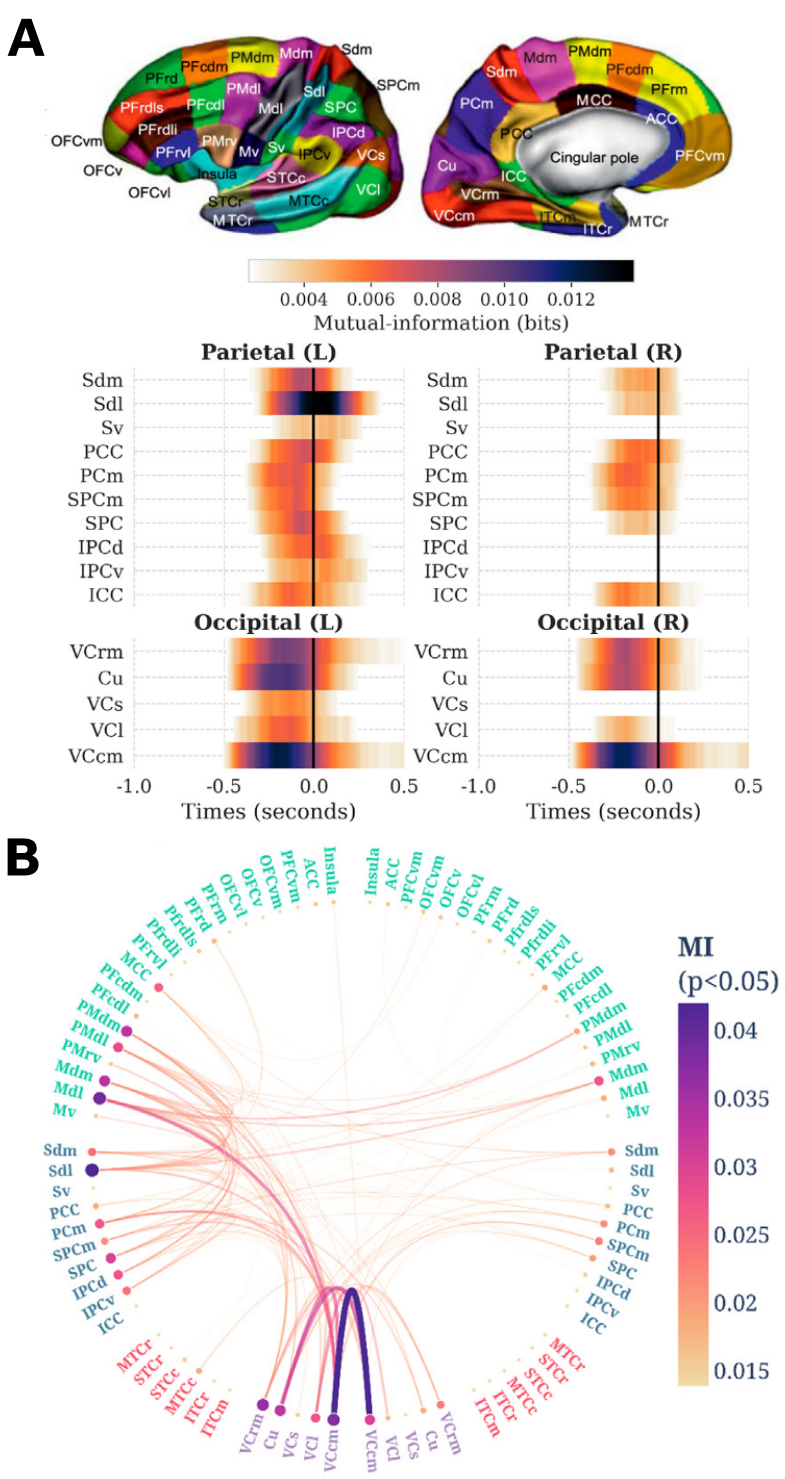
\includegraphics[width=0.40\textwidth]{figures/report/combrisson_2022_group_level_col.png}
    \caption{Group-level visuomotor-related local modulations of high-gamma activity (\textit{(A)} and connectivity fingerprint (\textit{(B)}}
    \label{fig_group_level}
\end{wrapfigure}

We recently proposed a unique statistical framework for performing group-level inferences, both at the local level of the brain region and at the network level \citep{combrisson2022grouplevel}. This framework combines several important features for robust discovery of cognitive brain networks : \textit{(i)} it allows identifying local activity or pairwise interactions between regions modulated according to an external variable (e.g. stimulus type or behavioural model like the prediction error or the surprise), \textit{(ii)} it supports both spatially uniform recordings (\ac{eeg}, \ac{meg}) and sparse recordings like \ac{ieeg}, \textit{(ii)} it encompasses cutting-edge measures of information from popular fields like \ac{ml} decoders or mutual-information from the \ac{it}, \textit{(iii)} it provides a flexible control of how to compensate for the inter-subjects variability using fixed- or random-effect models, \textit{(iv)} significance testing is assessed using non-parametric permutations with cluster-based correction and \textit{(v)} we provided an optimized Python implementation of the framework. 

% =======================================================================================
% =======================================================================================
%                                        VALORISATION
% =======================================================================================
% =======================================================================================

\section{Open-science, reproducibility and community-driven projects}

\subsection{Development of open-source software}

Visbrain \citep{combrisson2019visbrain}, Sleep \citep{combrisson2017sleep}. Tensorpac \citep{combrisson2020tensorpac}

\subsection{BrainHack events}

I contributed to the organization of hacking events \citep{gau2021brainhack}

\subsection{Good practices in M/EEG}

Contribution to a collective effort for defending \textbf{best practices in M/EEG} \citep{nisoGoodScientificPractice2022}

\newpage
\phantomsection
\addcontentsline{toc}{section}{References}

\begin{singlespace}
    \bibliography{refs}
\end{singlespace}

\end{document}